%@TheDoctorRAB
%standard white paper/preproposal format
%
%%%%%
%
%REFERENCES
%
%neup.bst - numbered citations in order of appearance, short author list with et al in reference section
%nsf.bst - numbered citations in order of appearance, full author list in references section
%standard.bst - citations with author last name with et al for more than 2 authors; full author list in references section
%ans.bst is for ANS only. 
%
%author = {Lastname, Firstname and Lastname, Firstname and Lastname, Firstname} for all bst formats
%bst renders the author list itself
%
%author = {{Nuclear Regulatory Commission}} if the author is an organization, institution, etc., and not people
%
%title = {{}} for all
%
%for all - use \citep{-} - [1] or (Borrelli, 2021) in the text
%standard.bst \cite{-} - Borrelli (2021) in the text
%standard.bst lists references alphabetically
%the rest list numerically
%
%
%%% slides 
%
%\citep{xxxnna} where the citation should go
%\blfootnote{\fontsize\cite{xxxnna}\fontsize\bibentry{xxxnna}} before \end{frame}
%
%
%%%%%

%%%%% presentation settings
\documentclass[aspectratio=1610,pdftex,dvipsnames,compress,xcolor={dvipsnames}]{beamer}
\usetheme{Boadilla}
\usecolortheme{seahorse}
\beamertemplatenavigationsymbolsempty
\addtobeamertemplate{footnote}{\hskip -2em}{} %pushes footnote to margin
\setbeamerfont{title}{series=\bfseries}
\setbeamertemplate{page number in head/foot}[framenumber] %just gives slide number; comment out for 1/7, 2/7...
\definecolor{BackGround}{RGB}{255,250,240}
\setbeamercolor{background canvas}{bg=BackGround}
%%%%%


%%%%% general 
%\documentclass[11pt,a4paper]{article}
%\usepackage[lmargin=1in,rmargin=1in,tmargin=1in,bmargin=1in]{geometry}
\usepackage[pagewise]{lineno} %line numbering
\usepackage{setspace}
\usepackage{ulem} %strikethrough - do not \sout{\cite{}}
\usepackage{graphicx}
\usepackage{mypythonhighlight,verbatim}
\usepackage{filecontents}
\usepackage{tablefootnote}
\usepackage{footnotehyper}
\usepackage{float}
%\usepackage{subfig}
\usepackage[yyyymmdd]{datetime} %date format
\renewcommand{\dateseparator}{.}
\graphicspath{{img/}} %path to graphics
\setcounter{secnumdepth}{5} %set subsection to nth level
\usepackage{needspace}
\usepackage[stable,hang,flushmargin]{footmisc} %footnotes in section titles and no indent; standard.bst
\usepackage[inline]{enumitem}
\setlist[itemize]{label=\textbullet}
\usepackage{boldline}
\usepackage{makecell}
\usepackage{booktabs}
\usepackage{amssymb}
\usepackage{gensymb}
\usepackage{amsmath,nicefrac}
\usepackage{physics}
\usepackage{lscape}
\usepackage{array}
\usepackage{chngcntr}
\usepackage{hyperref}
\hypersetup{colorlinks,linkcolor=black,citecolor=black,urlcolor=blue} 
%\usepackage{sectsty}
\usepackage{textcomp}
\usepackage{lastpage}
\usepackage{xargs} %for \newcommandx
\usepackage[colorinlistoftodos,prependcaption,textsize=tiny]{todonotes} %makes colored boxes for commenting
\usepackage{soul}
\usepackage{color}
\usepackage{marginnote}
\usepackage[figure,table]{totalcount}
\usepackage[capitalise]{cleveref}
\usepackage{microtype} %improves typography for pdf
\usepackage[pdftex,dvipsnames]{colortbl} %change font color
%%%%%


%%%%% tikz
\usepackage{pgf}
\usepackage{tikz} % required for drawing custom shapes
\usetikzlibrary{shapes,arrows,automata,trees}
%%%%%


%%%%% fonts
\usepackage{times}
%\renewcommand{\sfdefault}{ubuntu}
%arial - uncomment next two lines
%\usepackage{helvet}
%\renewcommand{\familydefault}{\sfdefault}
%%%%%


%%%%% references
%\usepackage[round,semicolon]{natbib} %for (Borrelli 2021; Clooney 2019) - standard.bst 
\usepackage[numbers,sort&compress]{natbib} %for [1-3] - nsf.bst, neup.bst
\setlength{\bibsep}{7pt} %sets space between references
%\renewcommand{\bibsection}{} %suppresses large 'references' heading
%\renewcommand\bibpreamble{\vspace{\baselineskip}} %sets spacing after heading if not using default references heading
%%%%%


%%%%% tables and figures
\usepackage{longtable} %need to put label at top under caption then \\ - use spacing
\usepackage{tablefootnote}
\usepackage{tabularx}
\usepackage{multirow}
\usepackage{tabto} %general tabbed spacing
\usepackage{pdfpages}
\usepackage{wrapfig} %wraps figures around text
\setlength{\intextsep}{0.00mm}
\setlength{\columnsep}{1.00mm}
\usepackage[singlelinecheck=false,labelfont=bf]{caption}
\usepackage{subcaption}
\captionsetup[table]{justification=justified,skip=5pt,labelformat={default},labelsep=period,name={Table}} %sets a space after table caption
\captionsetup[figure]{justification=justified,skip=5pt,labelformat={default},labelsep=period,name={Figure}} %sets space above caption, 'figure' format
\captionsetup[wrapfigure]{justification=centering,aboveskip=0pt,belowskip=0pt,labelformat={default},labelsep=period,name={Fig.}} %sets space above caption, 'figure' format
\captionsetup[wraptable]{justification=centering,aboveskip=0pt,belowskip=0pt,labelformat={default},labelsep=period,name={Table}} %sets space above caption, 'figure' format
%%%%%


%%%%% watermark
%\usepackage[firstpage,vpos=0.63\paperheight]{draftwatermark}
%\SetWatermarkText{\shortstack{DRAFT\\do not distribute}}
%\SetWatermarkScale{0.20}
%%%%%


%%%%% cross referencing files
%\usepackage{xr} %for revisions - will cross reference from one file to here
%\externaldocument{/path/to/auxfilename} %aux file needed
%%%%%


%%%%% toc and glossaries
\usepackage[toc,title]{appendix}
\usepackage[acronym,nomain,nonumberlist]{glossaries}
\makenoidxglossaries
%\usepackage{titlesec,titletoc}
%\renewcommand{\thepart}{ARTICLE \Roman{part}} %puts the label into the command so \thelabel will carry through
%\renewcommand{\thesection}{\arabic{section}} %puts the label into the command so \thelabel will carry through
%\titleformat{\part}{\normalfont\large\bfseries}{\thepart}{}{}[]
%\titlespacing*\part{0pt}{0.95\baselineskip}{0.75\baselineskip}
%\titleformat{\section}[runin]{\normalfont\large\bfseries}{\thesection}{-1em}{}[.]
%\titlespacing*\section{0pt}{0.65\baselineskip}{0.55\baselineskip}
%\titleformat{\subsection}[runin]{\normalfont\normalsize\bfseries}{\thesubsection}{-1em}{}[.]
%\titlespacing*\subsection{0pt}{0.50\baselineskip}{0.35\baselineskip}
%\titleformat{\paragraph}[runin]{\normalfont\normalsize\bfseries\itshape}{\theparagraph}{-1em}{}[.]
%\titlespacing*\paragraph{0pt}{0.45\baselineskip}{0.25\baselineskip}
%\titleformat{\subparagraph}[runin]{\normalfont\normalsize\itshape}{\thesubparagraph}{-1em}{}[.]
%\titlespacing*\subparagraph{0pt}{0.40\baselineskip}{0.25\baselineskip}
%\titleformat{\paragraph}[hang]{\normalfont\normalsize\bfseries}{\theparagraph}{5pt}{}[]
%\titlespacing*\paragraph{0pt}{0.50\baselineskip}{0.25\baselineskip}
%\titleformat{\subparagraph}[runin]{\normalfont\normalsize\itshape}{\thesubparagraph}{-1em}{}[.]
%\titlespacing*\subparagraph{0pt}{0.40\baselineskip}{0.20\baselineskip}
%%%%%


%%%%% editing
\newcommand{\edit}[1]{\textcolor{blue}{#1}} %shortcut for changing font color on revised text
\newcommand{\fn}[1]{\footnote{#1}} %shortcut for footnote tag
\newcommand*\sq{\mathbin{\vcenter{\hbox{\rule{.3ex}{.3ex}}}}} %makes a small square as a separator $\sq$
%\newcommand{\sk}[1]{\sout{#1}} %shortcut for default strikethrough - do not sk through citep
\newcommand\sk{\bgroup\markoverwith{\textcolor{red}{\rule[0.5ex]{1pt}{1pt}}}\ULon} %strikethrough with red line; not in \section{}
%\st{} does strikethrough using soul package but does not like acronyms
\newcommand{\blucell}{\cellcolor{aliceblue}} %use to shade in table cell
\newcommand{\grycekk}{\cellcolor{lightgray}} %use to shade in table cell
\newcommand{\whicell}{\cellcolor{antiquewhite}} %use to shade in table cell
%%%%%


%%%%% colors
%http://latexcolor.com/
%https://en.wikibooks.org/wiki/LaTeX/Colors#:~:text=black%2C%20blue%2C%20brown%2C%20cyan,be%20available%20on%20all%20systems.
\definecolor{aliceblue}{rgb}{0.94, 0.97, 1.0}
\definecolor{antiquewhite}{rgb}{0.98, 0.92, 0.84}
\definecolor{lightmauve}{rgb}{0.86, 0.82, 1.0}
\definecolor{brilliantlavender}{rgb}{0.96, 0.73, 1.0}
\definecolor{brandeisblue}{rgb}{0.0, 0.44, 1.0}
\definecolor{darkmidnightblue}{rgb}{0.0, 0.2, 0.4}

\newcommand{\x}{\cellcolor{aliceblue}} %use to shade in table cell
\newcommand{\y}{\cellcolor{lightgray}} %use to shade in table cell
\newcommand{\z}{\cellcolor{antiquewhite}} %use to shade in table cell
%%%%%


%%%%% acronyms
\newcommand{\acf}{\acrfull} %full acronym
\newcommand{\acl}{\acrlong} %long acronym
\newcommand{\acs}{\acrshort} %short acronym

\newcommand{\acfp}{\acrfullpl} %full acronym plural
\newcommand{\aclp}{\acrlongpl} %long acronym plural
\newcommand{\acsp}{\acrshortpl} %short acronym plural
%%%%%


%%%%% todonotes
\newcommandx{\cmt}[2][1=]{\todo[author=\textbf{STRUCTURE},tickmarkheight=0.15cm,linecolor=red,backgroundcolor=red!25,bordercolor=black,#1]{#2}}
\newcommandx{\con}[2][1=]{\todo[author=\textbf{CONTENT},tickmarkheight=0.15cm,linecolor=brilliantlavender,backgroundcolor=brilliantlavender,bordercolor=black,#1]{#2}}
\newcommandx{\rab}[2][1=]{\todo[noline,author=\textbf{RAB},backgroundcolor=Plum!25,bordercolor=black,#1]{#2}}


%\newcommandx{\jon}[2][1=]{\todo[noline,author=\textbf{ATTN: Johnson},backgroundcolor=blue!25,bordercolor=black,#1]{#2}}
%\newcommandx{\han}[2][1=]{\todo[noline,author=\textbf{ATTN: Haney},backgroundcolor=OliveGreen!25,bordercolor=black,#1]{#2}}
%\newcommandx{\rab}[2][1=]{\todo[author=\textbf{RAB},tickmarkheight=0.15cm,linecolor=Plum,backgroundcolor=Plum!25,bordercolor=black,#1]{#2}}
%\newcommandx{\han}[2][1=]{\todo[author=\textbf{ATTN: Haney},tickmarkheight=0.15cm,linecolor=OliveGreen,backgroundcolor=OliveGreen!25,bordercolor=OliveGreen,#1]{#2}}
%\newcommandx{\jon}[2][1=]{\todo[author=\textbf{ATTN: Johnson},tickmarkheight=0.15cm,linecolor=blue,backgroundcolor=blue!25,bordercolor=blue,#1]{#2}}


% highlighting 
\DeclareRobustCommand{\hlc}[1]{{\sethlcolor{LimeGreen}\hl{#1}}}
\makeatletter
    \if@todonotes@disabled
    \newcommand{\hlh}[2]{#1}
    \else
    \newcommand{\hlh}[2]{\han{#2}\hlc{#1}}
    \fi
    \makeatother

\DeclareRobustCommand{\hld}[1]{{\sethlcolor{CornflowerBlue}\hl{#1}}}
\makeatletter
    \if@todonotes@disabled
    \newcommand{\hlj}[2]{#1}
    \else
    \newcommand{\hlj}[2]{\jon{#2}\hld{#1}}
    \fi
    \makeatother

\DeclareRobustCommand{\hlf}[1]{{\sethlcolor{lightmauve}\hl{#1}}}
\makeatletter
    \if@todonotes@disabled
    \newcommand{\hlb}[2]{#1}
    \else
    \newcommand{\hlb}[2]{\rab{#2}\hlf{#1}}
    \fi
    \makeatother
%%%%%


%%%%% table alignments
\newcolumntype{L}[1]{>{\raggedright\let\newline\\\arraybackslash\hspace{0pt}}m{#1}} %uses \raggedright with m,p{} in table column
\newcolumntype{C}[1]{>{\centering\let\newline\\\arraybackslash\hspace{0pt}}m{#1}} %uses \raggedright with m,p{} in table column
\newcolumntype{R}[1]{>{\raggedleft\let\newline\\\arraybackslash\hspace{0pt}}m{#1}} %uses \raggedright with m,p{} in table column
%%%%%


%%%%% table contents
\makeatletter
\renewcommand\tableofcontents{%
    \@starttoc{toc}%
}
\makeatother

\makeatletter
\renewcommand\listoffigures{%
    \@starttoc{lof}%
}
\makeatother

\makeatletter
\renewcommand\listoftables{%
    \@starttoc{lot}%
}
\makeatother

\makeatletter
\newcommand*\ftp{\fontsize{16.5}{17.5}\selectfont}
\makeatother
%%%%%


%%%%% user commands
\newcommand\blfootnote[1]{%
  \begingroup
  \renewcommand\thefootnote{}\footnote{#1}%
  \addtocounter{footnote}{-1}%
  \endgroup
}

\makeatletter
\renewcommand{\@biblabel}[1]{#1.\hfill} %bibliography ordered list has numbers left flush
\makeatother
%%%%%

%%%%% archived section commands - use titlesec
%\makeatletter
%\renewcommand\section{%
%    \@startsection{section}{1}{\z@ }{0.50\baselineskip}{0.25\baselineskip}
%    {\large \normalfont \bfseries}}%

%\makeatletter
%\renewcommand\paragraph{%
%    \@startsection{paragraph}{4}{\z@ }{0.55\baselineskip}{-1em}
%    {\normalfont \normalsize \bfseries}}%

%\makeatletter
%\renewcommand\subparagraph{%
%    \@startsection{subparagraph}{5}{\z@ }{0.40\baselineskip}{-1em}
%    {\normalfont \normalsize \itshape }}%

%\makeatletter
%\renewcommand\subsection{%
%    \@startsection{subsection}{2}{\z@ }{0.45\baselineskip}{0.25\baselineskip}
%    {\large \normalfont \bfseries}}%
%%%%%


%%%%% header and footer
%\usepackage{fancyhdr}
%\pagestyle{fancy}
%\fancyhf{} %move page number to bottom right
%\renewcommand{\headrulewidth}{0pt} %set line thickness in header; uncomment as is to remove line
%\lhead{\scriptsize Name}
%\lhead{\scriptsize PNUCENE-D-22-xxxxx}
%\chead{\scriptsize \textit{PhD White Paper Project Proposal}}
%\rhead{\scriptsize \today}
%\rfoot{\thepage}
%%%%%


%%%%%%% citations
%\begin{filecontents}{references.bib}
%\end{filecontents}
%%%%%%%


%%%%% acronyms
% alphabetical ordering is automated
\newacronym{nrs}{NRHES}{Nuclear Renewable Hybrid Energy System}
\newacronym{ahp}{AHP}{Analytical Hierarchy Process}
\newacronym{inl}{INL}{Idaho National Laboratory}
\newacronym{orl}{ORNL}{Oak Ridge National Laboratory}
\newacronym{anl}{ANL}{Argonne National Laboratory}
\newacronym{npp}{NPP}{Nuclear Power Plant}
\newacronym{smr}{SMR}{Small Modular Reactor}
\newacronym{ump}{UAMPS}{Utah Associated Municipal Power Systems}
\newacronym{nus}{NuScale}{NuScale Power, LLC}
\newacronym{nrc}{NRC}{United States Nuclear Regulatory Commission}
\newacronym{epri}{EPRI}{Electric Power Research Institute}
\newacronym{nerc}{NERC}{North American Electric Reliability Corporation}
\newacronym{ci}{CI}{Consistency Index}
\newacronym{cr}{CR}{Consistency Ratio}
\newacronym{htse}{HTSE}{High Temperature Steam Electrolysis}
\newacronym{lwr}{LWR}{Light Water Reactor}
\newacronym{eia}{EIA}{U.S. Energy Information Administration}
\newacronym{oer}{OER}{Online Educational Resource}
\newacronym{lms}{LMS}{Learning Management System}
\newacronym{cps}{CPS}{Cyber-Physical Systems}
\newacronym{nsf}{NSF}{National Science Foundation}
\newacronym{wsc}{WSC}{Western Services Corporation}
\newacronym{cae}{CAES}{Center for Advanced Energy Studies}
\newacronym{hsl}{HSSL}{Human System Simulation Laboratory}
\newacronym{pwr}{PWR}{Pressurized Water Reactor}
\newacronym{bwr}{BWR}{Boiling Water Reactor}
\newacronym{roi}{ROI}{Return on Investment}
\newacronym{ic}{I\&C}{Instrumentation \& Controls}
\newacronym{mwe}{MWe}{Megawatts-electric}
\newacronym{ics}{ICS}{Industrial Control Systems}
\newacronym{sca}{SCADA}{Supervisory Control and Data Acquisition}
\newacronym{ip}{IP}{Internet Protocol}
\newacronym{udp}{UDP}{User Datagram Protocol}
\newacronym{tva}{TVA}{Tennessee Valley Authority}
\newacronym{plc}{PLC}{Programmable Logic Controller}
\newacronym{vfd}{VFD}{Variable Frequency Drive}
\newacronym{khp}{KHNP}{Korean Hydro \& Nuclear Power Co., Ltd}
\newacronym{onl}{ORNL}{Oak Ridge National Laboratory}
\newacronym{jcp}{JCPOA}{Joint Comprehensive Plan of Action}
\newacronym{mim}{MITM}{Man in the Middle}
\newacronym{dos}{DDoS}{Distributed Denial of Service}
\newacronym{tcp}{TCP/IP}{Transmission Control Protocol/Internet Protocol}
\newacronym{dnp}{DNP3}{Distributed Network Protocol 3}
\newacronym{pra}{PRA}{Probabilistic Risk Assessment}
\newacronym{cs}{CS}{Critical System}
\newacronym{loc}{LOCA}{Loss of Coolant Accident}
\newacronym{hmi}{HMI}{Human Machine Interface}
\newacronym{pha}{PHA}{Preliminary Hazards Analysis}
\newacronym{bol}{BOL}{Beginning-of-Life}
\newacronym{eol}{EOL}{End-of-Life}
\newacronym{mol}{MOL}{Middle-of-Life}
\newacronym{imu}{IMUNES}{Integrated Multiprotocol Network Emulator/Simulator}
\newacronym{ccc}{CCC}{Computing Community Consortium}
\newacronym{neu}{NEUP}{Nuclear Energy University Program}
\newacronym{doe}{DOE}{United States Department of Energy}
\newacronym{nei}{NEI}{Nuclear Energy Institute}
\newacronym{nit}{NITRD}{Networking Information Technology Research \& Development Program}
\newacronym{rcs}{RCS}{Reactor Cooling System}
\newacronym{con}{IC}{Initial Condition}
\newacronym{csi}{CSIS}{Center for Strategic \& International Studies}
\newacronym{pcap}{PCAP}{packet capture file}
\newacronym{dc}{DC}{Direct-Current}
\newacronym{ac}{AC}{Alternating-Current}
\newacronym{iff}{UIIF}{Idaho Falls Center for Higher Education}
\newacronym{snl}{SNL}{Sandia National Laboratory}
\newacronym{cie}{CIE}{Cyber-Informed Engineering}
\newacronym{cds}{CRDS}{Control Rod Drive System}
\newacronym{cdm}{CRDM}{Control Rod Drive Mechanism}
\newacronym{fma}{FMEA}{Failure Modes \& Effects Analysis}
\newacronym{rpn}{RPN}{Risk Priority Number}
\newacronym{scr}{SCR}{silicon controller rectifier}
\newacronym{hvc}{HVAC}{Heating, Ventilation \& Air Conditioning}
\newacronym{ttb}{TTB}{Time-to-Boil}
\newacronym{sis}{SIS}{Safety Instrumented System}
\newacronym{ui}{UI}{University of Idaho}
\newacronym{ala}{ALARA}{As Low As Reasonably Achievable}
\newacronym{pdf}{PDF}{Probability Density Function}
\newacronym{cdf}{CDF}{Cumulative Distribution Function}
\newacronym{osa}{OSHA}{Occupational Safety and Health Administration}
\newacronym{haz}{HAZOP}{Hazard \& Operability Analysis}
%\newacronym{}{}{}
%%%%%

%%%%% spacing
%\onehalfspacing %linespacing
%\setstretch{1.05} %linespacing
%\spacing{1.25} %equivalent to 1.5 line spacing in Word
%%%%%


%%%%% linenumbering
%\linenumbers %toggle line numbers
%\pagewiselinenumbers %reset line numbers on new page
%\modulolinenumbers[1] %line numbering interval
%%%%%


%%%%% title page
\addtocounter{framenumber}{-1} %does not count the title slide in the slide count
\title[NE529 -- Risk Assessment]{NE529\\RISK ASSESSMENT\\Preliminary hazards analysis\\3}
\author[@TheDoctorRAB]{R. A. Borrelli}
\institute[]{
    \acl{ui}\\
    \vspace{0.10in}
    
\includegraphics[width=0.20\textwidth]{ne-logo.png}
    }
\date{\acl{iff}}
%%%%%

\begin{document}


%%%%% title page with no footer
{
    \setbeamertemplate{footline}{}
    \begin{frame}
        \titlepage
    \end{frame}
}
%%%%%


\begin{frame}{Learning objectives}
    \begin{enumerate}[series=outerlist,topsep=0pt,itemsep=15pt,leftmargin=*,label=(\arabic*)]
        \item[]Interpeting \acs{pha} within the context of risk assessment
        \item[]Applying \acs{pha} to engineering problems and work environment
        \item[]Developing a systematic approach to risk assessment
        \item[]Chapter 6 in the book
    \end{enumerate}
\end{frame}


\begin{frame}{Learning nodes}
    \begin{columns}[t]

        \begin{column}{0.50\textwidth}
            \begin{enumerate}[series=outerlist,topsep=0pt,itemsep=1pt,leftmargin=*,label=(\arabic*)]
                \item[]\textbf{Defining hazards}
                    \vspace{0.10in}
                \item[]\textbf{Risk assessment flowchart}
                    \vspace{0.10in}
                \item[]\textbf{Identifying hazards}
                    \vspace{0.10in}
                \item[]\textbf{\acs{osa}}
                    \vspace{0.10in}
                \item[]\textbf{\acs{pha} framework}
                \item[]Hazards
                \item[]Consequences
                \item[]Procedures
                    \vspace{0.10in}
                \item[]\textbf{Pyroprocessing example}
            \end{enumerate}
        \end{column}

        \begin{column}{0.50\textwidth}
            \begin{enumerate}[series=outerlist,topsep=0pt,itemsep=1pt,leftmargin=*,label=(\arabic*)]
                \item[]\hfill\textbf{Analysis methods}
                \item[]\hfill Forward
                \item[]\hfill Backward
                \item[]\hfill Top down
                \item[]\hfill Bottom up
                    \vspace{0.10in}
                \item[]\hfill\textbf{Lifecycle considerations}
                    \vspace{0.10in}
                \item[]\hfill\textbf{Preliminary risk quantification}
                \item[]\hfill Frequency estimation
                \item[]\hfill Consequence estimation
                    \vspace{0.10in}
                \item[]\hfill\textbf{Common cause failures}
                    \vspace{0.05in}
                \item[]\hfill\textbf{Visualizing risk}
                    \vspace{0.05in}
                \item[]\hfill\textbf{Hazard elimination}
                    \vspace{0.05in}
                \item[]\hfill\textbf{Criticisms}
            \end{enumerate}
        \end{column}

    \end{columns}
\end{frame}


\begin{frame}[plain]{}
    \centering\LARGE\textbf{What is a hazard?}
\end{frame}


\addtocounter{framenumber}{-1}
\begin{frame}{\acf{pha} is a semi-quantitative analysis tool}
    \begin{enumerate}[series=outerlist,topsep=0pt,itemsep=15pt,leftmargin=*,label=(\arabic*)]
        \item[]Line item tabular inventory of non trivial system hazards and countermeasures
        \item[]Best applied in the design and development stage  
        \item[]Early phase risk assessment tool
        \item[]Identify all potential hazards and intiating events that may lead to an accident
        \item[]Rank the identified events according to their severity  
        \item[]Can be drawn from the risk assessment matrix from before
    \end{enumerate}
\end{frame}


\begin{frame}{Identify required hazard controls and follow-up actions}
    \begin{enumerate}[series=outerlist,topsep=0pt,itemsep=11pt,leftmargin=*,label=(\arabic*)]
        \item[]Systematic process to identify hazards, prioritize, and propose mitigation
        \item[]Produce a Preliminary Hazard List
        \item[]Leading to deeper analytical tools
        \item[]Rapid risk ranking  
        \item[]Hazard identification
        \item[]\acf{fma}
        \item[]\acf{haz}
        \item[]Human error analysis
    \end{enumerate}
\end{frame}


\begin{frame}[plain]{}
    \centering\Large\textbf{Risk assessment requires continual refinement}
\end{frame}


\addtocounter{framenumber}{-1}
\begin{frame}{Overall risk assessment flowchart}
    \begin{figure}
        \centering
        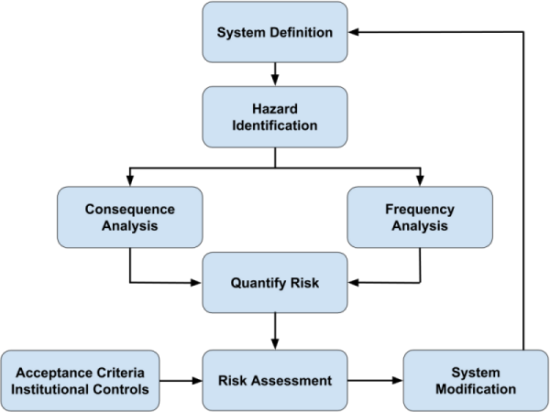
\includegraphics[width=0.70\textwidth]{chart.png}
%        \caption{}
    \end{figure}
\end{frame}


\begin{frame}{Identify the hazards in this office space}
    \begin{figure}
        \centering
        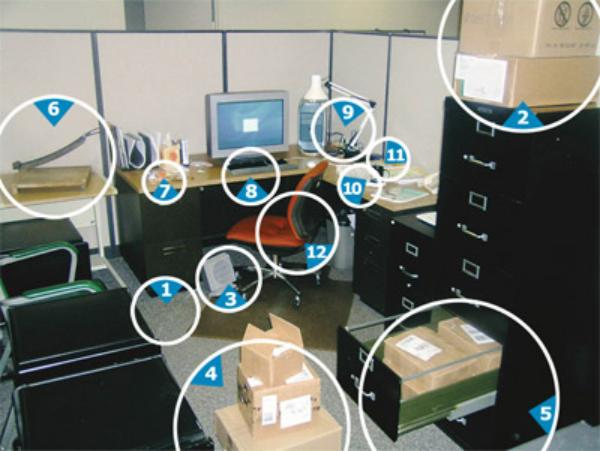
\includegraphics[width=0.70\textwidth]{office.space.jpg}
%        \caption{}
    \end{figure}
\end{frame}


\begin{frame}{}
    \begin{figure}
        \centering
        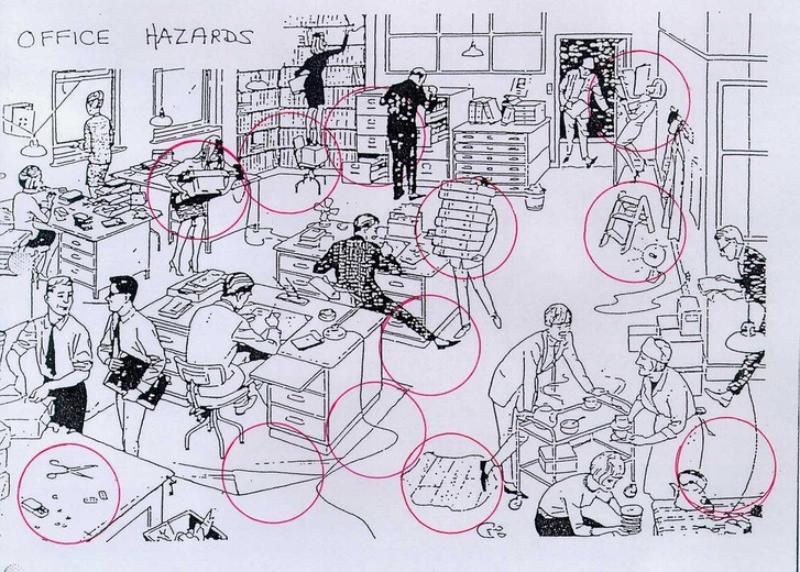
\includegraphics[width=0.80\textwidth]{workplace.jpg}
%        \caption{}
    \end{figure}
\end{frame}


\begin{frame}{Risk assessment is everyone's responsibility}
    \begin{figure}
        \centering
        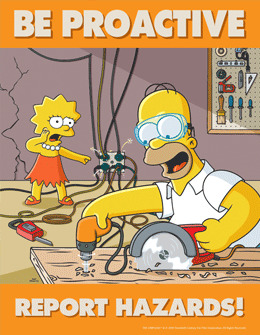
\includegraphics[width=0.40\textwidth]{simpsons.jpg}
%        \caption{}
    \end{figure}
\end{frame}


\begin{frame}[plain]{}
    \centering\Large\textbf{What are some hazards \acs{osa} might cite?}
\end{frame}


\addtocounter{framenumber}{-1}
\begin{frame}{\acs{osa} top 10 warehouse citations}
    \begin{enumerate}[series=outerlist,topsep=0pt,itemsep=5pt,leftmargin=*,label=(\arabic*)]
        \item Forklifts 
        \item Hazard communication
        \item Electrical -- wiring methods
        \item Electrical -- system design
        \item Guarding floor, wall openings, holes
        \item Exits
        \item Mechanical power transmission
        \item Lockout, tagout
        \item Respiratory protection
        \item Portable fire extinguishers
    \end{enumerate}
\end{frame}


\begin{frame}{}
    \begin{figure}
        \centering
        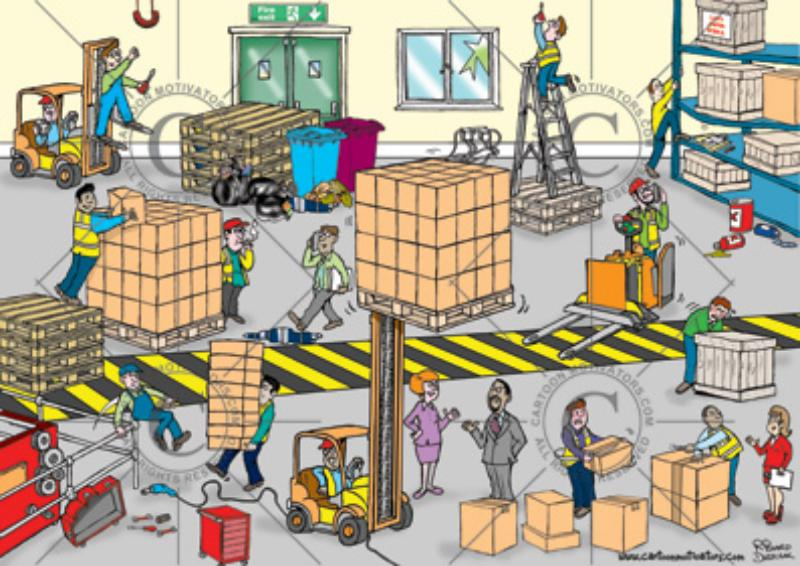
\includegraphics[width=0.80\textwidth]{warehouse.jpg}
%        \caption{}
    \end{figure}
\end{frame}


\begin{frame}{}
    \begin{figure}
        \centering
        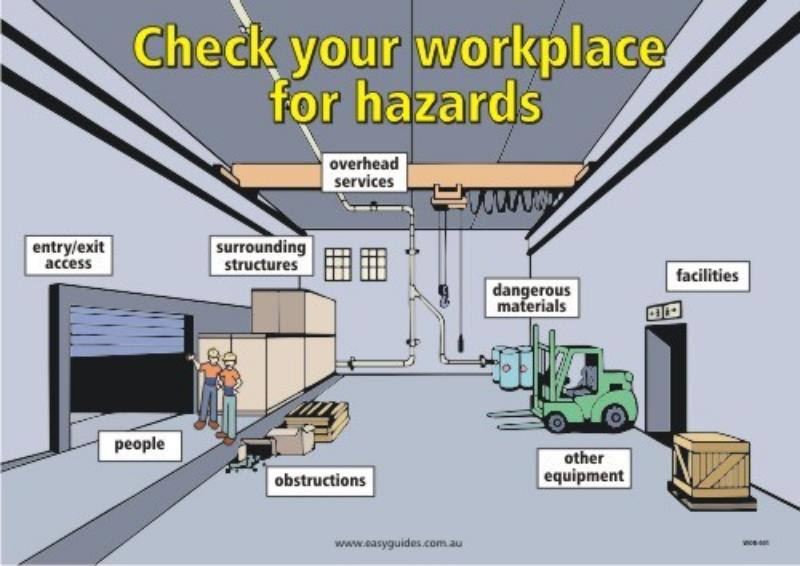
\includegraphics[width=0.80\textwidth]{loading.dock.jpg}
%        \caption{}
    \end{figure}
\end{frame}


\begin{frame}{}
    \begin{figure}
        \centering
        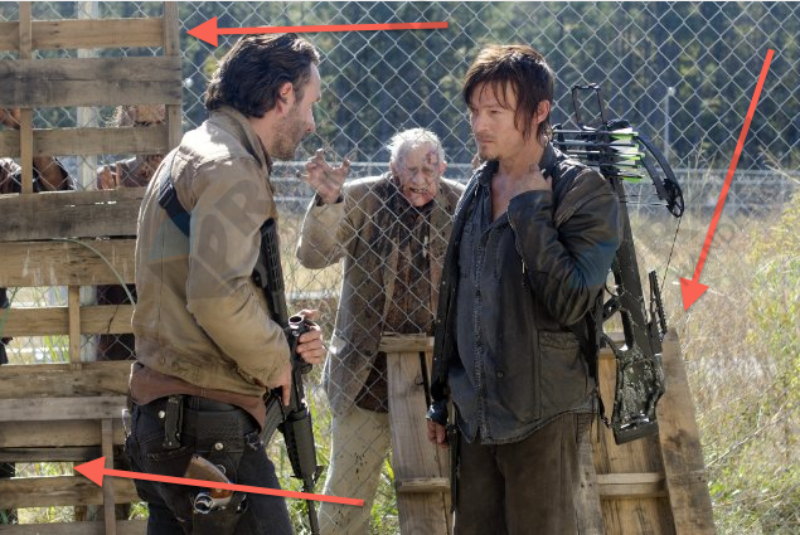
\includegraphics[width=0.80\textwidth]{the.walking.dead.jpg}
%        \caption{}
    \end{figure}
\end{frame}


\begin{frame}[plain]{}
    \centering\LARGE\textbf{\acs{pha} framework}
\end{frame}


\addtocounter{framenumber}{-1}
\begin{frame}{\href{https://uidaho.pressbooks.pub/riskassessment/chapter/preliminary-hazards-analysis/}{\acs{pha}} is used as an initial risk study in the early stages of the project}
    \begin{enumerate}[series=outerlist,topsep=0pt,itemsep=21pt,leftmargin=*,label=(\arabic*)]
        \item[]Initially developed by US Army
        \item[]`Army had half day, Mother!'
        \item[]Used to review process areas of energy released in uncontrolled manner
        \item[]Identify hazards and consequences
        \item[]Start as early as possible in system life cycle
    \end{enumerate}
\end{frame}


\begin{frame}{Adapt \acs{pha} to the system under study}
    \begin{enumerate}[series=outerlist,topsep=0pt,itemsep=7pt,leftmargin=*,label=(\arabic*)]
        \item[]Not everything is applicable to every system
        \item[]Identify hazardous components or system elements
        \item[]Facility related hazards and surrounding property
        \item[]Interfaces between system elements related to safety (software)
        \item[]Operational \& supporting equipment  
        \item[]Safety equipment and related safeguards
        \item[]Environmental \& operational constraints  
        \item[]Leading to potential malfunctions to system and components
    \end{enumerate}
\end{frame}


\begin{frame}[plain]{}
    \centering\LARGE\textbf{Hazards}
\end{frame}


\addtocounter{framenumber}{-1}
\begin{frame}{Identify potential hazards where energy may be released}
    \begin{columns}[c]

        \begin{column}{0.50\textwidth}
            \begin{enumerate}[series=outerlist,topsep=0pt,itemsep=11pt,leftmargin=*,label=(\arabic*)]
                \item[]Mechanical moving parts  
                \item[]Material incompatibilities  
                \item[]Nuclear radiation  
                \item[]Electromagnetic radiation (laser, radio, UV)  
                \item[]Collisions from movement of personnel, equipment, automation
            \end{enumerate}
        \end{column}

        \begin{column}{0.50\textwidth}
            \begin{enumerate}[series=outerlist,topsep=0pt,itemsep=11pt,leftmargin=*,label=(\arabic*)]
                \item[]Toxic materials, corrosive liquids; gases stored, generated  
                \item[]All sorts of deterioration  
                \item[]Subsonic or supersonic noise  
                \item[]Biological, bacterial growth  
                \item[]Human error  
                \item[]Software, network, cyber-based 
            \end{enumerate}
        \end{column}

    \end{columns}
\end{frame}


\begin{frame}{Identify hazardous states of a system as part of the conceptual design phase}
    \begin{enumerate}[series=outerlist,topsep=0pt,itemsep=7pt,leftmargin=*,label=(\arabic*)]
        \item[]Inputs
        \item[]Boundaries between the system(s)  
        \item[]System interaction and dependencies  
        \item[]System domain  
        \item[]System functionality for each component and holistically  
        \item[]Layout  
        \item[]Process flow  
        \item[]Output
    \end{enumerate}
\end{frame}


\begin{frame}{Identify where each hazard will occur}
    \begin{enumerate}[series=outerlist,topsep=0pt,itemsep=21pt,leftmargin=*,label=(\arabic*)]
        \item[]Significance
        \item[]Method to eliminate or mitigate
        \item[]How associated risk will be controlled
    \end{enumerate}
\end{frame}


\begin{frame}[plain]{}
    \centering\LARGE\textbf{Consequences}
\end{frame}


\addtocounter{framenumber}{-1}
\begin{frame}{Identify consequences that may occur from each hazard}
    \begin{enumerate}[series=outerlist,topsep=0pt,itemsep=9pt,leftmargin=*,label=(\arabic*)]
        \item[]Estimate frequency of hazards  
        \item[]Estimate of the severity of each event  
        \item[]Compare initial design concepts  
        \item[]Focus on important risk issues  
        \item[]You might be able to easily mitigate some events right at the start
        \item[]Consider \acs{pha} to be the base level of risk analysis  
        \item[]It is not sufficient but a necessary start
    \end{enumerate}
\end{frame}


\begin{frame}{Assign each consequence a severity categorization}
    \begin{enumerate}[series=outerlist,topsep=0pt,itemsep=21pt,leftmargin=*,label=(\arabic*)]
        \item[]Quantify frequency of each accident sequence
        \item[]Assign each hazard a preliminary random and systematic probability target
        \item[]Propose safety features needed during the design and development phase
        \item[]You want to be able to head off low risk that can be mitigated by design and high risk that needs more work 
    \end{enumerate}
\end{frame}


\begin{frame}[plain]{}
    \centering\LARGE\textbf{Procedures}
\end{frame}


\addtocounter{framenumber}{-1}
\begin{frame}{Identify procedures related to operations, testing, maintenance, system diagnostics, emergencies}
    \begin{enumerate}[series=outerlist,topsep=0pt,itemsep=11pt,leftmargin=*,label=(\arabic*)]
        \item[]Obtain potential related data cohorts  
        \item[]Reports, accident statistics, regulatory reviews if you know someone  
        \item[]Or existing systems and \acsp{pha}
        \item[]Bring in some experts for an outside review
        \item[]Model energy or material flow in the system and develop operational modes  
        \item[]Review facility technical specifications if they are available  
        \item[]Not so easy even though `qualitative'
    \end{enumerate}
\end{frame}


\begin{frame}{\acs{pha} is most effectively used during the initial development of a process and the procedures for performing that process}
    \begin{enumerate}[series=outerlist,topsep=0pt,itemsep=21pt,leftmargin=*,label=(\arabic*)]
        \item[]List the hazards and not to analyze each step in the procedure  
        \item[]Very top-level analysis, but when done properly, very useful for more comprehensive \acs{pra}
        \item[]Would we really need this with mature systems?
    \end{enumerate}
\end{frame}


\begin{frame}{}
    \begin{figure}
        \centering
        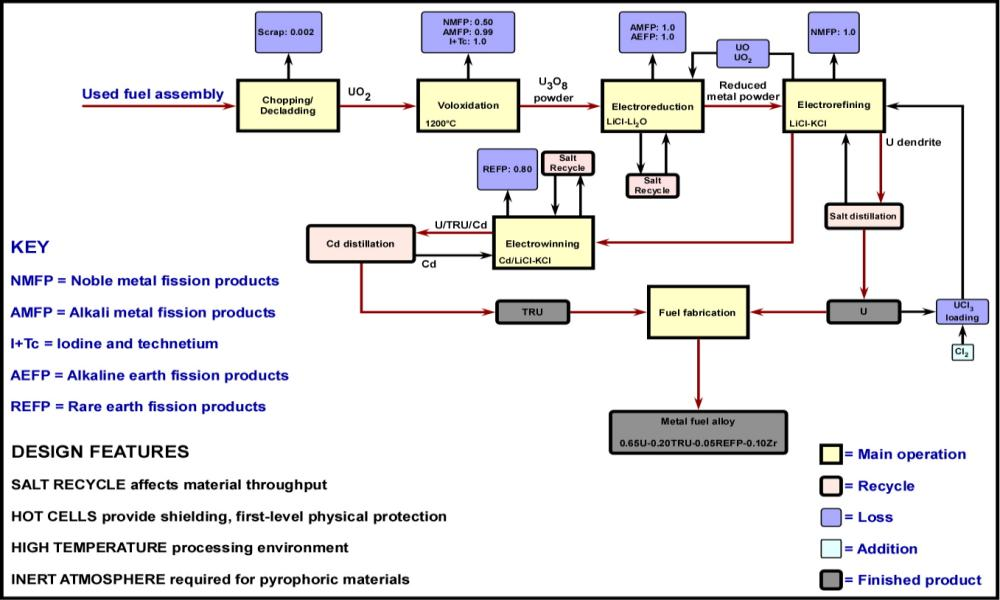
\includegraphics[width=0.80\textwidth]{pyroprocessing.flowsheet.jpg}
%        \caption{}
    \end{figure}
\end{frame}


\begin{frame}[plain]{}
    \centering\LARGE\textbf{Analysis methods}
\end{frame}


\begin{frame}[plain]{}
    \centering\LARGE\textbf{Forward}
\end{frame}


\addtocounter{framenumber}{-2}
\begin{frame}{Forward analysis identifies events then consequences}
    \begin{figure}
        \centering
        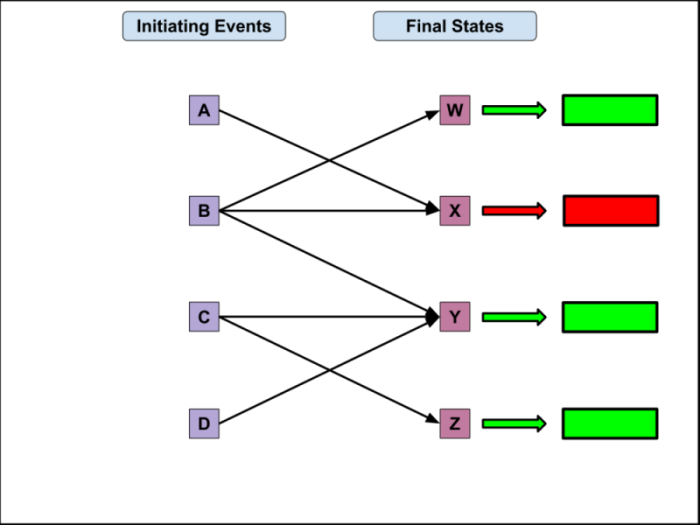
\includegraphics[width=0.70\textwidth]{forward.jpg}
%        \caption{}
    \end{figure}
\end{frame}


\begin{frame}[plain]{}
    \centering\LARGE\textbf{Backward}
\end{frame}


\addtocounter{framenumber}{-1}
\begin{frame}{Backward analysis identifies hazards to find events}
    \begin{figure}
        \centering
        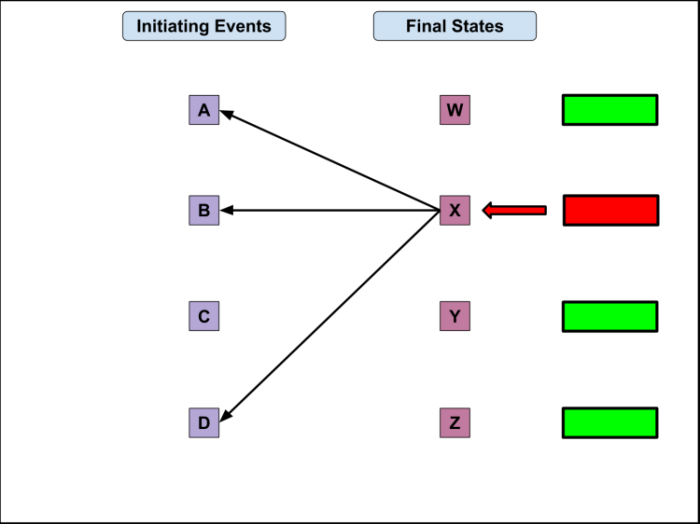
\includegraphics[width=0.70\textwidth]{backward.jpg}
%        \caption{}
    \end{figure}
\end{frame}


\begin{frame}[plain]{}
    \centering\LARGE\textbf{Top down}
\end{frame}


\addtocounter{framenumber}{-1}
\begin{frame}{Use top down analysis to decompose the events}
    \begin{figure}
        \centering
        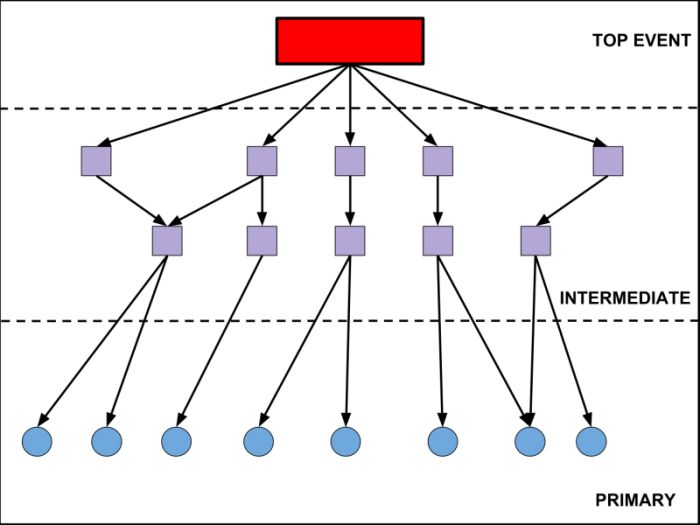
\includegraphics[width=0.70\textwidth]{top.down.jpg}
%        \caption{}
    \end{figure}
\end{frame}


\begin{frame}[plain]{}
    \centering\LARGE\textbf{Bottom up}
\end{frame}


\addtocounter{framenumber}{-1}
\begin{frame}{Use bottom up analysis to decompose the hazard}
    \begin{figure}
        \centering
        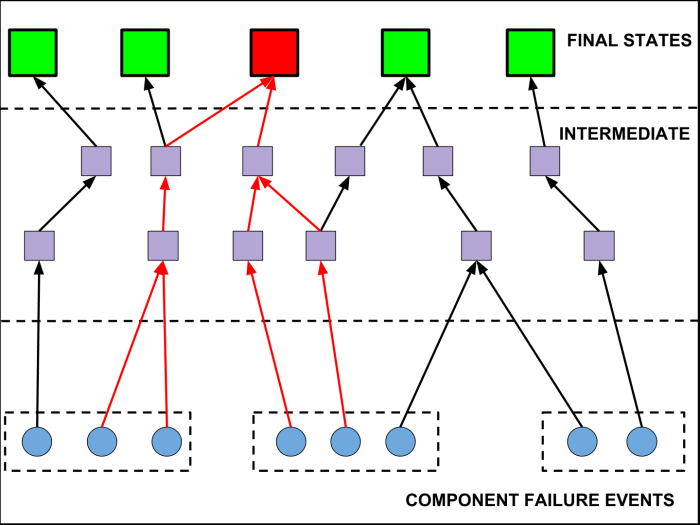
\includegraphics[width=0.70\textwidth]{bottom.up.jpg}
%        \caption{}
    \end{figure}
\end{frame}


\begin{frame}[plain]{}
    \centering\LARGE\textbf{Lifecycle considerations}
\end{frame}


\addtocounter{framenumber}{-1}
\begin{frame}{\acs{pha} should take place during different stages in the lifecycle}
    \begin{enumerate}[series=outerlist,topsep=0pt,itemsep=21pt,leftmargin=*,label=(\arabic*)]
        \item[]New facilities as part of design before committing resources
        \item[]During construction, things are going to come up that were not anticipated
        \item[]\begin{quote}We know what we know\\We know what we don't know\\We don't know what we don't know\end{quote}
        \item[]Operational readiness must be conducted prior to system start up
    \end{enumerate}
\end{frame}


\begin{frame}{Periodic analysis during operational lifetime}
    \begin{enumerate}[series=outerlist,topsep=0pt,itemsep=15pt,leftmargin=*,label=(\arabic*)]
        \item[]Maybe due to regulations
        \item[]Anytime there is a modification  
        \item[]Safety analysis at USA nuclear plants after Fukushima
        \item[]\acs{nrc} regulations for technical specification, performance based goals, best practices
        \item[]Finally, when decommissioning new hazards will arise
        \item[]Disposal of materials, chemicals, etc.
    \end{enumerate}
\end{frame}


\begin{frame}[plain]{}
    \centering\LARGE\textbf{Preliminary risk quantification}
\end{frame}


\begin{frame}[plain]{}
    \centering\LARGE\textbf{Frequency estimation}
\end{frame}


\addtocounter{framenumber}{-2}
\begin{frame}{Estimate probability of occurrence}
    \begin{enumerate}[series=outerlist,topsep=0pt,itemsep=3pt,leftmargin=*,label=(\arabic*)]
        \item[]$< 10^{-6}$ -- less than credible 
        \item[]Not expected during facility lifetime
            \vspace{0.10in}
        \item[]$10^{-6} - 10^{-4}$ -- credible and extremely unlikely
        \item[]Probably not occur during facility lifetime
            \vspace{0.10in}
        \item[]$10^{-4} - 10^{-2}$ -- credible and unlikely
        \item[]May occur once during facility lifetime
        \item[]Natural phenomena
        \item[]Trained worker error
            \vspace{0.10in}
        \item[]$10^{-2} - 10^{-1}$ -- very likely
        \item[]Events may often occur
    \end{enumerate}
\end{frame}


\begin{frame}{You can just guess at the start}
    \begin{enumerate}[series=outerlist,topsep=0pt,itemsep=21pt,leftmargin=*,label=(\arabic*)]
        \item[]Frequent -- occurs often
        \item[]Likely -- occurs several times
        \item[]Occasional -- occurs sporadically
        \item[]Seldom -- not negligible but unlikely
        \item[]Unlikely -- neglibible
    \end{enumerate}
\end{frame}


\begin{frame}[plain]{}
    \centering\LARGE\textbf{Consequence estimation}
\end{frame}


\addtocounter{framenumber}{-1}
\begin{frame}{Rank hazards in terms of qualitative consequences or severity}
    \begin{enumerate}[series=outerlist,topsep=0pt,itemsep=3pt,leftmargin=*,label=(\arabic*)]
        \item[]\textbf{Class I -- Negligible}
        \item[]Worst case effects cause less than minor injury, occupational illness, system damage
            \vspace{0.10in}
        \item[]\textbf{Class II -- Marginal effects}
        \item[]Worst case effects cause minor occupational illness, system damage
            \vspace{0.10in}
        \item[]\textbf{Class III -- Critical}
        \item[]Worst case effects cause severe (nondisabling) personnel injury, severe occupational illness, major system damage
            \vspace{0.10in}
        \item[]\textbf{Class IV -- Catastrophic}
        \item[]Worst case effects cause death, disabling injury, system loss
            \vspace{0.25in}
        \item[]Most reliable solution is to eliminate source of hazard
    \end{enumerate}
\end{frame}


\begin{frame}[plain]{}
    \centering\LARGE\textbf{Common cause failures}
\end{frame}


\addtocounter{framenumber}{-1}
\begin{frame}{Beware common cause events or multiple consequences}
    \begin{enumerate}[series=outerlist,topsep=0pt,itemsep=21pt,leftmargin=*,label=(\arabic*)]
        \item[]Different events may lead to similar consequences
        \item[]Ranking hazards needs a normalized metric
        \item[]So severity must be carefully determined 
        \item[]Consequences should be characterized as precisely or descriptively as possible 
        \item[]Estimate the frequency that initiating event produces a specific consequence 
        \item[]This means that for each initiating event, there might be several consequences with associated frequencies
    \end{enumerate}
\end{frame}


\begin{frame}{Example for a typical warehouse environment}
    \begin{enumerate}[series=outerlist,topsep=0pt,itemsep=21pt,leftmargin=*,label=(\arabic*)]
        \item[]Worker (sober) falls off a ladder
        \item[]Risk = low severity but moderate frequency
        \item[]Could be fatal, but low frequency, not negligible
        \item[]Both should be considered in \acs{pha}
        \item[]How can this risk be mitigated?
        \item[]Maybe you have a separate section where fatalities are considered
        \item[]How else could this be classified?
    \end{enumerate}
\end{frame}


\begin{frame}[plain]{}
    \centering\LARGE\textbf{Visualizing risk}
\end{frame}


\addtocounter{framenumber}{-1}
\begin{frame}{Clearer comparisons can be made now}
    \begin{figure}
        \centering
        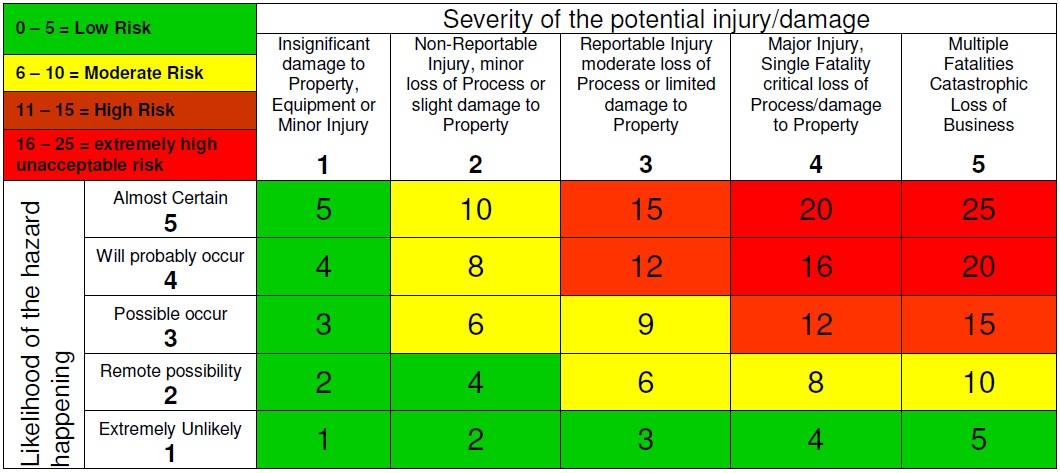
\includegraphics[width=0.90\textwidth]{matrix.jpg}
%        \caption{}
    \end{figure}
\end{frame}


\begin{frame}{}
    \begin{figure}
        \centering
        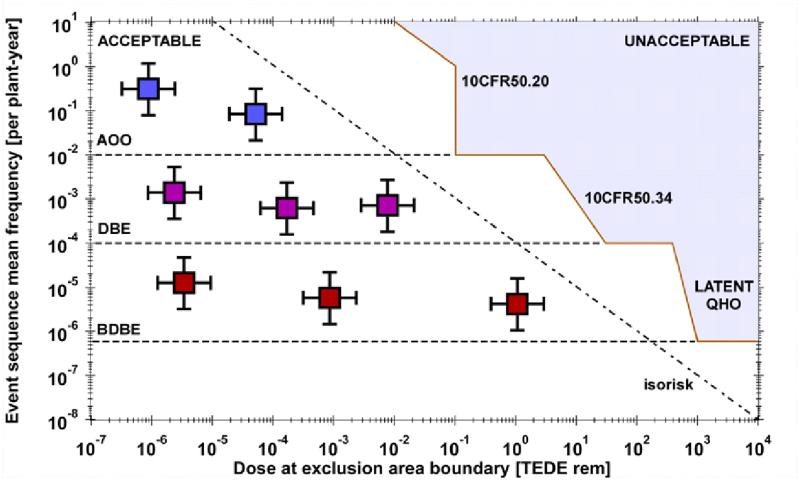
\includegraphics[width=0.90\textwidth]{farmer.jpg}
%        \caption{}
    \end{figure}
\end{frame}


\begin{frame}[plain]{}
    \centering\LARGE\textbf{Hazard reduction}
\end{frame}


\addtocounter{framenumber}{-1}
\begin{frame}{How can hazards be eliminated?}
    \begin{enumerate}[series=outerlist,topsep=0pt,itemsep=1pt,leftmargin=*,label=(\arabic*)]
        \item[]\textbf{Substitution}
        \item[]Use safe materials  
        \item[]Simple hardware devices may be safer than using a computer
        \item[]No technological imperative that says we MUST use computers to control dangerous devices  
        \item[]Introducing new technologies increases unknowns
            \vspace{0.05in}
        \item[]\textbf{Simplify}
        \item[]Limit process states  
        \item[]Easily understood and readable  
        \item[]Interactions between components are limited and straightforward  
        \item[]Code includes only minimum features and capability required by system  
        \item[]No unnecessary, undocumented features, unused executable code  
        \item[]Worst case timing is determinable  
        \item[]Design so that structural decomposition matches functional decomposition
    \end{enumerate}
\end{frame}


\begin{frame}{How else can hazards be eliminated?}
    \begin{enumerate}[series=outerlist,topsep=0pt,itemsep=1pt,leftmargin=*,label=(\arabic*)]
        \item[]\textbf{Decouple}
        \item[]Tightly coupled system is one that is highly interdependent  
        \item[]Failure or unplanned behavior in one can rapidly affect status of others  
        \item[]System accidents caused by unplanned interactions  
        \item[]Coupling creates increased number of interfaces and potential interactions
            \vspace{0.15in}
        \item[]\textbf{Passive safeguards}
        \item[]Fail to a safe state
            \vspace{0.15in}
        \item[]\textbf{Redundancy and diversity}
            \vspace{0.15in}
        \item[]\textbf{Human error}
    \end{enumerate}
\end{frame}


\begin{frame}[plain]{}
    \centering\LARGE\textbf{Criticisms}
\end{frame}


\addtocounter{framenumber}{-1}
\begin{frame}{What's so good about \acs{pha}?}
    \begin{enumerate}[series=outerlist,topsep=0pt,itemsep=15pt,leftmargin=*,label=(\arabic*)]
        \item[]Helps ensure that the system is safe
        \item[]Modifications are less expensive and easier to implement in earlier design stages  
        \item[]Decreases design time by reducing the number of surprises  
        \item[]Identifies and provides a log of primary system hazards and corresponding risks
        \item[]Provides systematic evaluation early enough to allow for design mitigation (Rokkasho)
        \item[]Provides information to management to make decisions to allocate resources to reduce risk
        \item[]Provides relatively quick review of most significant system risks
    \end{enumerate}
\end{frame}


\begin{frame}{What's not so good about \acs{pha}?}
    \begin{enumerate}[series=outerlist,topsep=0pt,itemsep=5pt,leftmargin=*,label=(\arabic*)]
        \item[]Hazards must be foreseen by the analysts  
        \item[]Effects of interactions between hazards are not easily recognized  
        \item[]You don't know what you don't know  
        \item[]Can fail to assess risks well of combined hazards of common failure modes  
        \item[]Then underrepresent overall system risk
        \item[]Insufficient or inappropriate targets chosen; assessment is flawed
        \item[]Garbage in = garbage out  
        \item[]Wrong assumptions for unknown data, etc.
        \item[]Too many targets, \acs{pha} becomes large and costly  
        \item[]Which misses the point
    \end{enumerate}
\end{frame}


\begin{frame}[plain]{}
    \begin{figure}
        \centering
        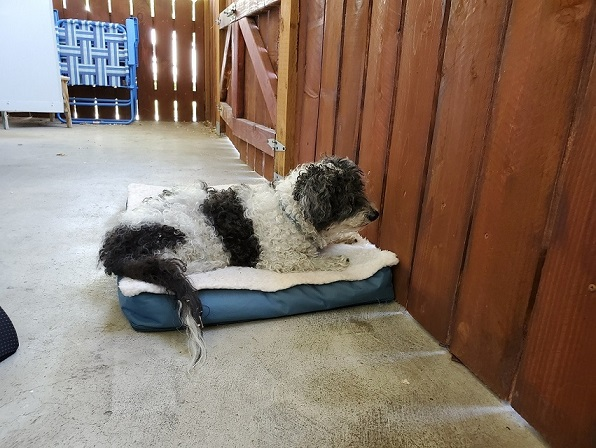
\includegraphics[width=0.65\textwidth]{final.jpg}
%        \caption{}
    \end{figure}
\end{frame}


%%%%%%%
%\begin{frame}{}
%    \begin{columns}
%
%        \begin{column}{0.50\textwidth}
%            \begin{enumerate}[series=outerlist,topsep=0pt,itemsep=21pt,leftmargin=*,label=(\arabic*)]
%                \item[]
%                \item[]
%            \end{enumerate}
%        \end{column}
%
%        \begin{column}{0.50\textwidth}
%            \begin{enumerate}[series=outerlist,topsep=0pt,itemsep=21pt,leftmargin=*,label=(\arabic*)]
%                \item[]
%                \item[]
%            \end{enumerate}
%        \end{column}
%
%    \end{columns}
%\end{frame}

%    \begin{figure}
%        \centering
%        \includegraphics[width=0.75\textwidth]{wsc.png}
%        \caption{\acs{wsc}}
%    \end{figure}


%\begin{frame}{References}
%    \bibliographystyle{nsf}
%    \footnotesize
%    \bibliography{references}
%\end{frame}
%%%%%%%


\end{document}
